\chapter{Further work on the model}
\label{secondPhaseOfModelingCyberInsurance} 

So far our model have only considered the effects of direct connections, but in this part we will introduce the effects of indirect connections. When a node connects to a new node, the change in payoff is not just a fixed variable as earlier, but also dependent on the connections already established by the other node.

In the earlier model network effects the nodes experiences, arises from their neighbours only. I.e. when a node establish a connection the change in utility is only dependent on fixed variables, and non dependent of the rest of the network.
In the previous models the utility for each node where only affected by direct variables such as $\beta$. In a real world scenario a node will be strongly affected by network externalities. Our idea is based on the paper from Jackson and Wolinsky \cite{jackson1996strategic} and a network formation game in \cite{jackson2005survey}. 

\section{The connection game}
We consider a connection game where the network effects are dependent on the whole network.  Meaning, in addition to the benefit from the direct connection, a node will also benefit from "the friends of the friend", and "the friends of the friends of the friend" etc. This is achieved by letting the payoff be calculated relative to the distance between the nodes. The network externality $\beta$ is now dependent on the number of hops to the node e.g. the benefit of a direct connection is $\beta$, the benefit of a friend of a friend is $\beta^2$ etc. We want the benefit to be decreasing with the distance, so we need this limitation: $0<\beta<1$ on $\beta$. 

\begin{figure}[h]
\centering
  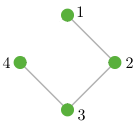
\includegraphics[width=0.2\linewidth]{../Figures/connectionGame.png}
  \caption{\label{fig:connectionGame} Four nodes interconnected with each other.}
\end{figure}
lets consider the network shown in \ref{fig:connectionGame}. Node 1 in the network will get a benefit of $\beta+\beta^{2}+\beta^{3}$ by having the connection with node 2. For this network to make sense, it is important to also include some cost of having direct connections. This is done as in earlier models, every node pay a cost for direct connections, but no cost for indirect connections. Thus the total payoff for a node is:

\begin{equation}
\sum_{j\neq i}^{} \beta_{ij}^{d(ij)} - \sum_{j:ij\in g}^{} {c}_{ij}, 
\label{connecetionGame}
\end{equation}

where $d(ij)$ represents the shortest path between node $i $ and node $j $, and ${c}_{ij}$ represents node i's cost of establishing a link between the two nodes. To simplify the model we choose a symmetric connection process where $\beta$ and $c$ is set to a fixed global value. 

In the paper \cite{jackson1996strategic}, they analyze the stability and efficiency of a network like this. An efficient network means ending up with a network where the sum of every nodes payoff is maximized. The optimal network is of course both efficient and stable, but as we shall see there are some conflicts between efficiency and stability. In the paper they found that an efficient network is:
\begin{enumerate}
\item \textit{a complete graph $g^N$ if $c<\beta - \beta^2$,}
\item \textit{a star encompassing every node if $\beta - \beta^2 < c < \beta + \frac{(N-2)}{2}\beta^2$,}
\item \textit{an empty network(no links) if $\beta + \frac{(N-2)}{2}\beta^2 < c$.}
\end{enumerate}

Proposition 1, says that when the cost of insuring a link is low, it would be more beneficial for every node, to have a direct connection to another node, compared to an indirect connection.
Proposition 3, when the insurance cost is high, it is best to not have any connections at all.

The most efficient structure is created in the intermediate cost of insuring links, and ends up in a star structure which encompasses every node. A star structure have the characteristics of minimizing the average path length and uses the minimum number of links($N-1$) required for including every node to the network. 
Indisputable this structure provides the highest overall payoff for the network, but this network is not necessarily stable, as we will show later on.

\subparagraph{Pairwise stability:(HVERTFALL ISH )}
A graph is pairwise stable if:
 \begin{enumerate}
\item \textit{No node want to delete a link he is involved in.}
\item \textit{If there exists a node who want to add a link, then the node on the other end of the link do not want to establish this link.}
\end{enumerate} 
The limitations of pairwise stability is that we only consider one link and one pair of nodes at a time.


When analyzing the stability of the network, by using pairwise stability, Jackson and Wolinsky found four different conditions of stability:

\begin{enumerate}
\item \textit{a pairwise stable network consists of at most one (non-empty) component,}
\item \textit{if $c<\beta - \beta^2$, the unique pairwise stable network will be a complete graph $g^N$, }
\item \textit{if $\beta - \beta^2 <c < \beta $, a star encompassing every node will be pairwise stable, although not necessarily the unique pairwise stable graph,}
\item \textit{if $\beta < c$ , any pairwise stable network which is nonempty is such that each player has at least two links and thus be inefficient. }
\end{enumerate}
We see that the stability condition 2, is the same as the efficiency condition 1, and thus if this condition is fulfilled, the network is both stable and efficient. 
Condition 3 shows us why the efficient star network is not necessarily  stable. If $\beta \geq c <   \beta + \frac{(N-2)}{2}\beta^2$ then the efficient network will be a star, but it is not stable.

It should be noticed that it is more beneficial for a node to operate as a leaf node compared to being a center node, due to the cost of direct connection. In a star structure, a leaf node will only have to pay the cost of the link to the center node, and will benefit indirectly for each node connected to the center node. The center node will benefit from each new connection, however, the payoff will only be $\beta - c$ for each connection. 

SKRIV Om simulering.

To solve the problem, one has to compensate the center node for the extra cost of creating network externalities. As described in the previous model considering bulk insurance discount, the insurance company could implement a bonus which lowers the cost for each new connection. This would lower the extra cost for the center node significantly, as it is expected that the number of nodes might be high and therefore result in a significant discount. 
Using the discount calculation from previous models, we end up with the following equation for the star topology:

\begin{equation}
\beta-\beta^2<\frac{i_{l}}{i+1}< \beta
\end{equation}



where $i $ is represent the number of connections a node have established. 

Although this enhancement ensures that the cost for the center node is lowered, it does not guarantee that the center node is fully compensated. To accomplish this, the insurance companies have to directly compensate the center nodes. As described earlier a star topology will create a super critical payoff, and a star topology would be beneficial for the insurance companies. Hence the insurance companies will have incentive to compensate the center nodes additionally to enable the star structure to be generated. 




